\documentclass[12pt]{article}

% Any percent sign marks a comment to the end of the line

% Every latex document starts with a documentclass declaration like this
% The option dvips allows for graphics, 12pt is the font size, and article
%   is the style

\usepackage[pdftex]{graphicx}
\usepackage{url}
\usepackage[hidelinks]{hyperref}


\usepackage{pdfpages}

% These are additional packages for "pdflatex", graphics, and to include
% hyperlinks inside a document.

\setlength{\oddsidemargin}{0.25in}
\setlength{\textwidth}{6.5in}
\setlength{\topmargin}{0in}
\setlength{\textheight}{8.5in}

% These force using more of the margins that is the default style

\begin{document}

% Everything after this becomes content
% Replace the text between curly brackets with your own

\title{LifeMAX: Technical Specification}
\date{\today}

\maketitle

\section{Points and Leaderboard}

\begin{enumerate}
\item \textbf{Jason}: Add score \emph{(score:integer)} to User object.  Every task the user completes is worth 1 point.
\item \textbf{Charles}: Create view for \emph{Leaderboard}.  This tab should be accessed from the sidebar.  The leaderboard should display the rankings of only the people in your friends list.  It is sorted from most points to least points.
\item \textbf{Charles}: Add to sidebar (needs icon).

\begin{figure}[htbp]
    \centering
    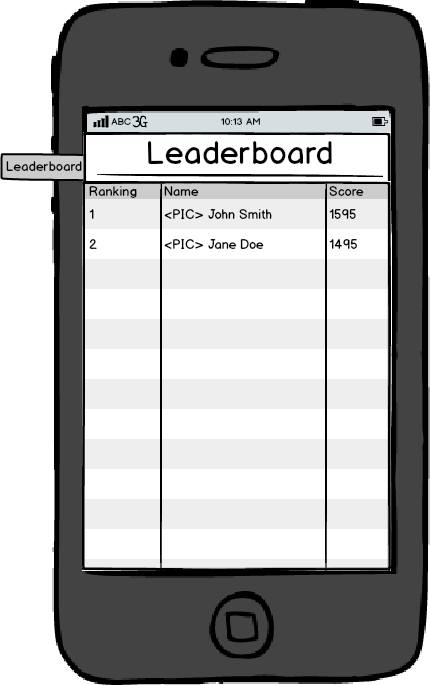
\includegraphics[width=0.35\textwidth]{leaderboard.png}
    \caption{Mockup of Leaderboard Screen.}
    \label{fig:leaderboard}
\end{figure}

\end{enumerate}

\section{Suggestions Page}
\begin{enumerate}
\item Remove "Max Suggests tasks from the News Feed.
	\begin{itemize}
	\item \textbf{Jason}: Prevent rendering of Max events from the API.
	\item \textbf{Charles}: Remove render code from the News Feed.
	\end{itemize}
\item \textbf{Charles}: Create view for \emph{Suggestions}.  This tab should be accessed from the sidebar.  The view should display all "Max Suggests" goals.  Remove the words "Max Suggests" from each goal since the page is dedicated only for those goals.  Keep the green bar and the LifeMAX logo.
\item \textbf{Charles}: Add suggestions to sidebar (needs icon).
\item \textbf{Delete Goals}:
	\begin{itemize}
	\item \textbf{Jason}: Build backend infrastructure to allow users to belong to goals they no longer want to see.
	\item \textbf{Charles}: Add a button to delete or hide a goal.
	\end{itemize}
\end{enumerate}

\section{Modify Goals Page}
\begin{enumerate}
\item \textbf{Charles}: Remove the transparent background on task names in the news feed.
\item \textbf{Charles}: Remove the "done" and "add" links from the bottom of goals that aren't your goals.
\item Description Field:
	\begin{itemize}
	\item \textbf{Jason}: Add description field into task table in database.
	\item \textbf{Charles}: Add field into task creation and task display views to allow users to create and view descriptions for each goal they set.
	\end{itemize}
	
\begin{figure}[htbp]
    \centering
    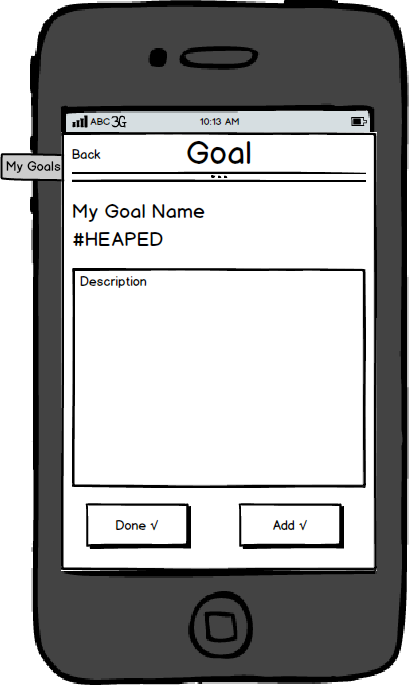
\includegraphics[width=0.35\textwidth]{view_description.png}
    \caption{Allow users to view descriptions.}
    \label{fig:view_desc}
\end{figure}
	
\item \textbf{Charles}: Allow users to tap on goals.  If you own a goal, it takes you to the page to edit that goal.  If it is not your goal, it takes you to a view that displays information on that goal, and allows you to add it as one of your own goals.
\end{enumerate}
\end{document}     
     
     
     
     
     
     
